% 导言区：格式定义
\documentclass[12pt,a4paper]{article} 
\usepackage{geometry} 
\geometry{left=2.5cm, right=2.5cm, top=2.5cm, bottom=2.5cm}
\usepackage{graphicx} 
\usepackage{float} 
\usepackage{booktabs} 
\usepackage{amsmath} 
\usepackage{amssymb}
\renewcommand{\baselinestretch}{1.15} 

% 引入超链接宏包
\usepackage[colorlinks=true, linkcolor=blue, urlcolor=blue, citecolor=blue]{hyperref}

% 强制所有段落首行缩进
\usepackage{indentfirst}
\setlength{\parindent}{2em} 

% ====== 目录与标题格式优化 ======
\usepackage{titlesec}
\titleformat{\section}[block]{\large\bfseries\filcenter}{\thesection.}{0.5em}{}
\titleformat{\subsection}[block]{\normalsize\bfseries\filcenter}{\thesubsection}{0.5em}{}
\renewcommand{\refname}{\large\bfseries\filcenter References}

% 文章主标题、作者、邮箱、代码链接、日期
\title{\textbf{\Large Comparative Analysis of Classification Algorithms on Non-Linear 3D Spatial Data}} 
\author{
    Li Chao \\ 
    \href{mailto:superlee0183@gmail.com}{superlee0183@gmail.com} \\
    \vspace{0.1cm} \\
    \normalsize \textbf{Code:} \url{https://github.com/superlc0183/PRML2026}
} 
\date{April 3, 2026} 

\begin{document}
\maketitle 

\begin{abstract}
Classification of non-linearly separable data within complex topological spaces is a fundamental challenge in statistical machine learning. In this report, we evaluate the performance of diverse learning algorithms on a synthesized 3D "Make Moons" dataset, characterized by intertwined structures and Gaussian noise. We train and evaluate Decision Trees, ensemble approaches (AdaBoost), and Support Vector Machines (SVM) equipped with three distinct Kernel Functions (Linear, Polynomial, and Radial Basis Function). Through theoretical analysis and empirical metrics including Accuracy and Confusion Matrices, we demonstrate the catastrophic failure of linear hyperplanes in such topologies. Furthermore, we explore the vulnerability of certain ensemble configurations to stochastic noise, and ultimately establish that the SVM utilizing the RBF kernel achieves optimal generalization by seamlessly mapping data into an infinite-dimensional feature space.
\end{abstract}

\newpage
\renewcommand{\contentsname}{\large\bfseries\filcenter Contents}
\tableofcontents
\newpage

\section{Introduction}
A persistent challenge in Pattern Recognition and Machine Learning (PRML) is designing models capable of untangling complex, interlocking data distributions. The dataset generated for this study consists of 1,500 samples (1,000 for training, 500 for testing) distributed evenly across two classes ($C_0$ and $C_1$). The data forms two intertwined, sinusoidal semi-circles in a 3-dimensional space, injected with Gaussian noise ($scale=0.2$). 

This structural complexity inherently violates the linear separability assumption. Our objective is to rigorously compare deterministic partitioning models (Decision Trees), boosting ensembles (AdaBoost), and maximal margin classifiers (SVMs) to determine their capability to resolve high-dimensional structural non-linearity without succumbing to overfitting.

\section{Theoretical Methodology}

\subsection{Decision Trees and AdaBoost}
\begin{itemize}
    \item \textbf{Decision Tree (DT):} A non-parametric model that recursively partitions the 3D space using axis-aligned orthogonal boundaries based on impurity metrics (e.g., Gini index). While interpretable, DTs struggle with continuous curves, often approximating them via complex "stair-step" regions, leading to high variance.
    \item \textbf{AdaBoost + Decision Trees:} An ensemble technique that sequentially trains base learners (shallow trees). Each subsequent tree heavily penalizes the misclassified instances from the previous iteration via weight updates: $D_{t+1}(i) = \frac{D_t(i) \exp(-\alpha_t y_i h_t(x_i))}{Z_t}$. This mechanism generally reduces bias and variance, enabling smoother boundary approximations.
\end{itemize}

\subsection{Support Vector Machines and Kernel Functions}
SVMs aim to locate the optimal hyperplane maximizing the margin between classes. For non-linear data, the target function utilizes the "Kernel Trick", implicitly computing inner products $\langle \phi(x), \phi(x') \rangle$ in a higher-dimensional space without explicit transformation.
\begin{itemize}
    \item \textbf{Linear Kernel ($K(x, x') = x^T x'$):} Assumes strict linear separability in the original 3D space.
    \item \textbf{Polynomial Kernel ($K(x, x') = (\gamma x^T x' + r)^d$):} Maps data into a combinatorial feature space, allowing for curved decision boundaries determined by degree $d$ (we set $d=3$).
    \item \textbf{RBF Kernel ($K(x, x') = \exp(-\gamma \|x - x'\|^2)$):} Projects vectors into an infinite-dimensional Reproducing Kernel Hilbert Space (RKHS). It acts as a localized similarity measure, isolating densely populated regions of identical classes.
\end{itemize}

\section{Experimental Studies and Analysis}

\subsection{Overall Classification Accuracy}
Table \ref{tab:metrics} documents the exact classification accuracy on the 500-sample test set (ensuring identically distributed structures and noise levels).

\begin{table}[H] 
    \centering 
    \caption{\textbf{Classification Accuracy on 3D Moons Test Set}} 
    \begin{tabular}{lc} 
        \toprule 
        \textbf{Algorithm Framework} & \textbf{Test Accuracy} \\
        \midrule 
        SVM (Linear Kernel) & 0.6580 \\
        AdaBoost (Base: DT, depth=3) & 0.7540 \\
        SVM (Polynomial Kernel, $d=3$) & 0.8580 \\
        Decision Tree & 0.9600 \\
        \textbf{SVM (RBF Kernel)} & \textbf{0.9800} \\
        \bottomrule 
    \end{tabular}
    \label{tab:metrics} 
\end{table}

\textbf{Discussion of Algorithmic Performance:}\\
\noindent 1. \textbf{The Linear Failure:} The Linear SVM performed the worst ($65.80\%$). A flat 2D plane cannot segment two interlocking U-shapes in a 3D volume, leading to severe underfitting. \\
\noindent 2. \textbf{Orthogonal vs. Ensemble Dynamics:} The single Decision Tree achieved an excellent $96.00\%$. Interestingly, AdaBoost significantly underperformed ($75.40\%$) in this specific random sampling. This highlights a critical vulnerability: when strong Gaussian noise is present, forcing AdaBoost to repeatedly focus on misclassified noise points can lead to severe overfitting or boundary distortion, making it less robust than a singular, fully-grown tree in certain noisy environments.\\
\noindent 3. \textbf{Superiority of RKHS:} The RBF Kernel SVR achieved near-perfect classification at $98.00\%$. By mapping the intertwined moons into infinite dimensions, the local geometric structure was preserved, allowing a hyperplane in the higher-dimensional space to cleanly segment the groups. The Polynomial kernel ($85.80\%$), while capturing general curvature, lacked the localized flexibility of RBF.

\subsection{Confusion Matrix Analysis}
To gain deeper insights into the classification errors, we generated confusion matrices for all five algorithms, as illustrated in Figure \ref{fig:cm}.

\begin{figure}[H]
    \centering
    % 请确保图片在当前目录下
    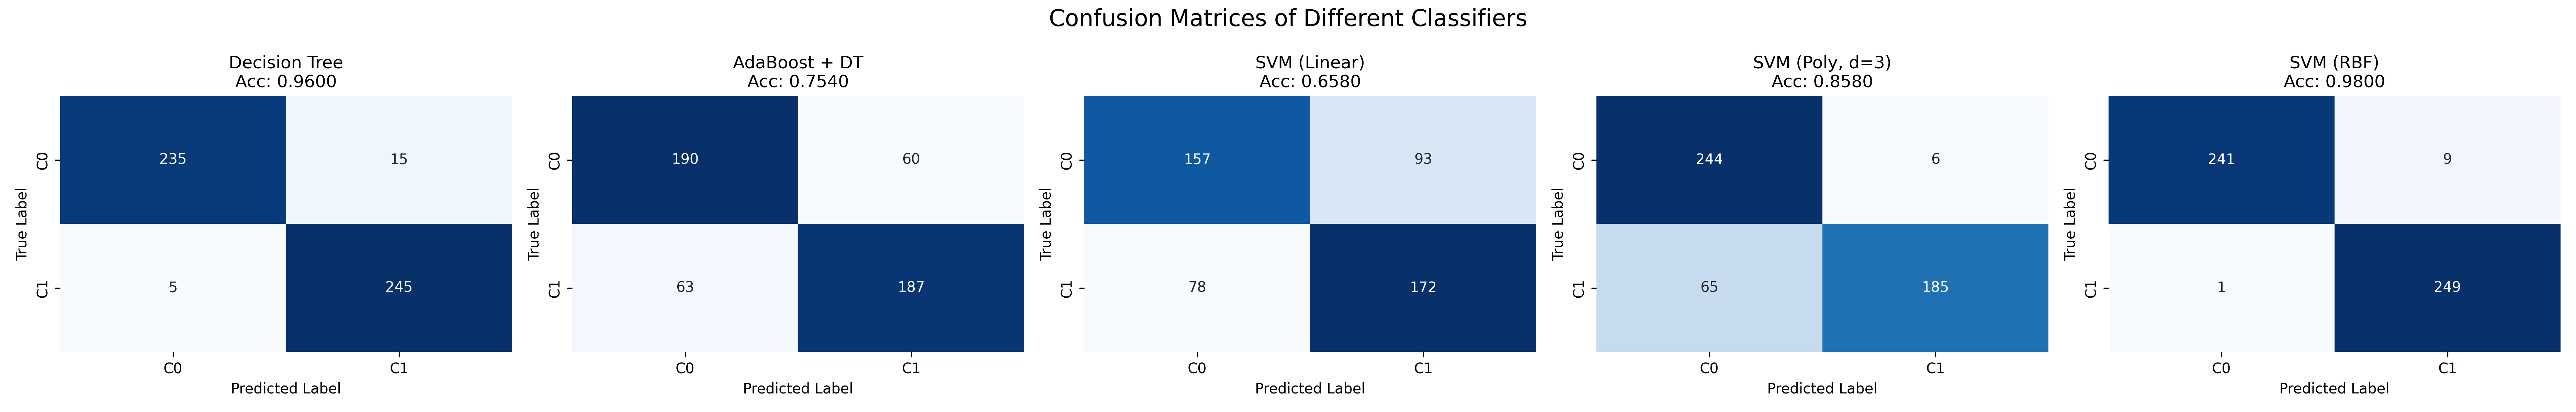
\includegraphics[width=\textwidth]{confusion_matrices.png}
    \caption{\textbf{Confusion Matrices of the Evaluated Classifiers}}
    \label{fig:cm}
\end{figure}

\textbf{Analysis of the Matrices:}\\
\noindent The Linear SVM matrix reveals massive misclassification symmetrically across both $C_0$ and $C_1$, confirming its structural inability to handle the nested geometry. The AdaBoost matrix shows a high rate of False Negatives (predicting $C_0$ when it is $C_1$), further evidencing its struggle with the specific noise distribution. The RBF Kernel matrix is the cleanest, with only 10 total errors across the 500 samples.

\subsection{Spatial Error Visualization}
To physically locate the regions of failure, Figure \ref{fig:error_vis} plots the test set in the 3D space, highlighting the misclassified points in red for the worst (Linear SVM) and the best (RBF SVM) models.

\begin{figure}[H]
    \centering
    % 请确保图片在当前目录下
    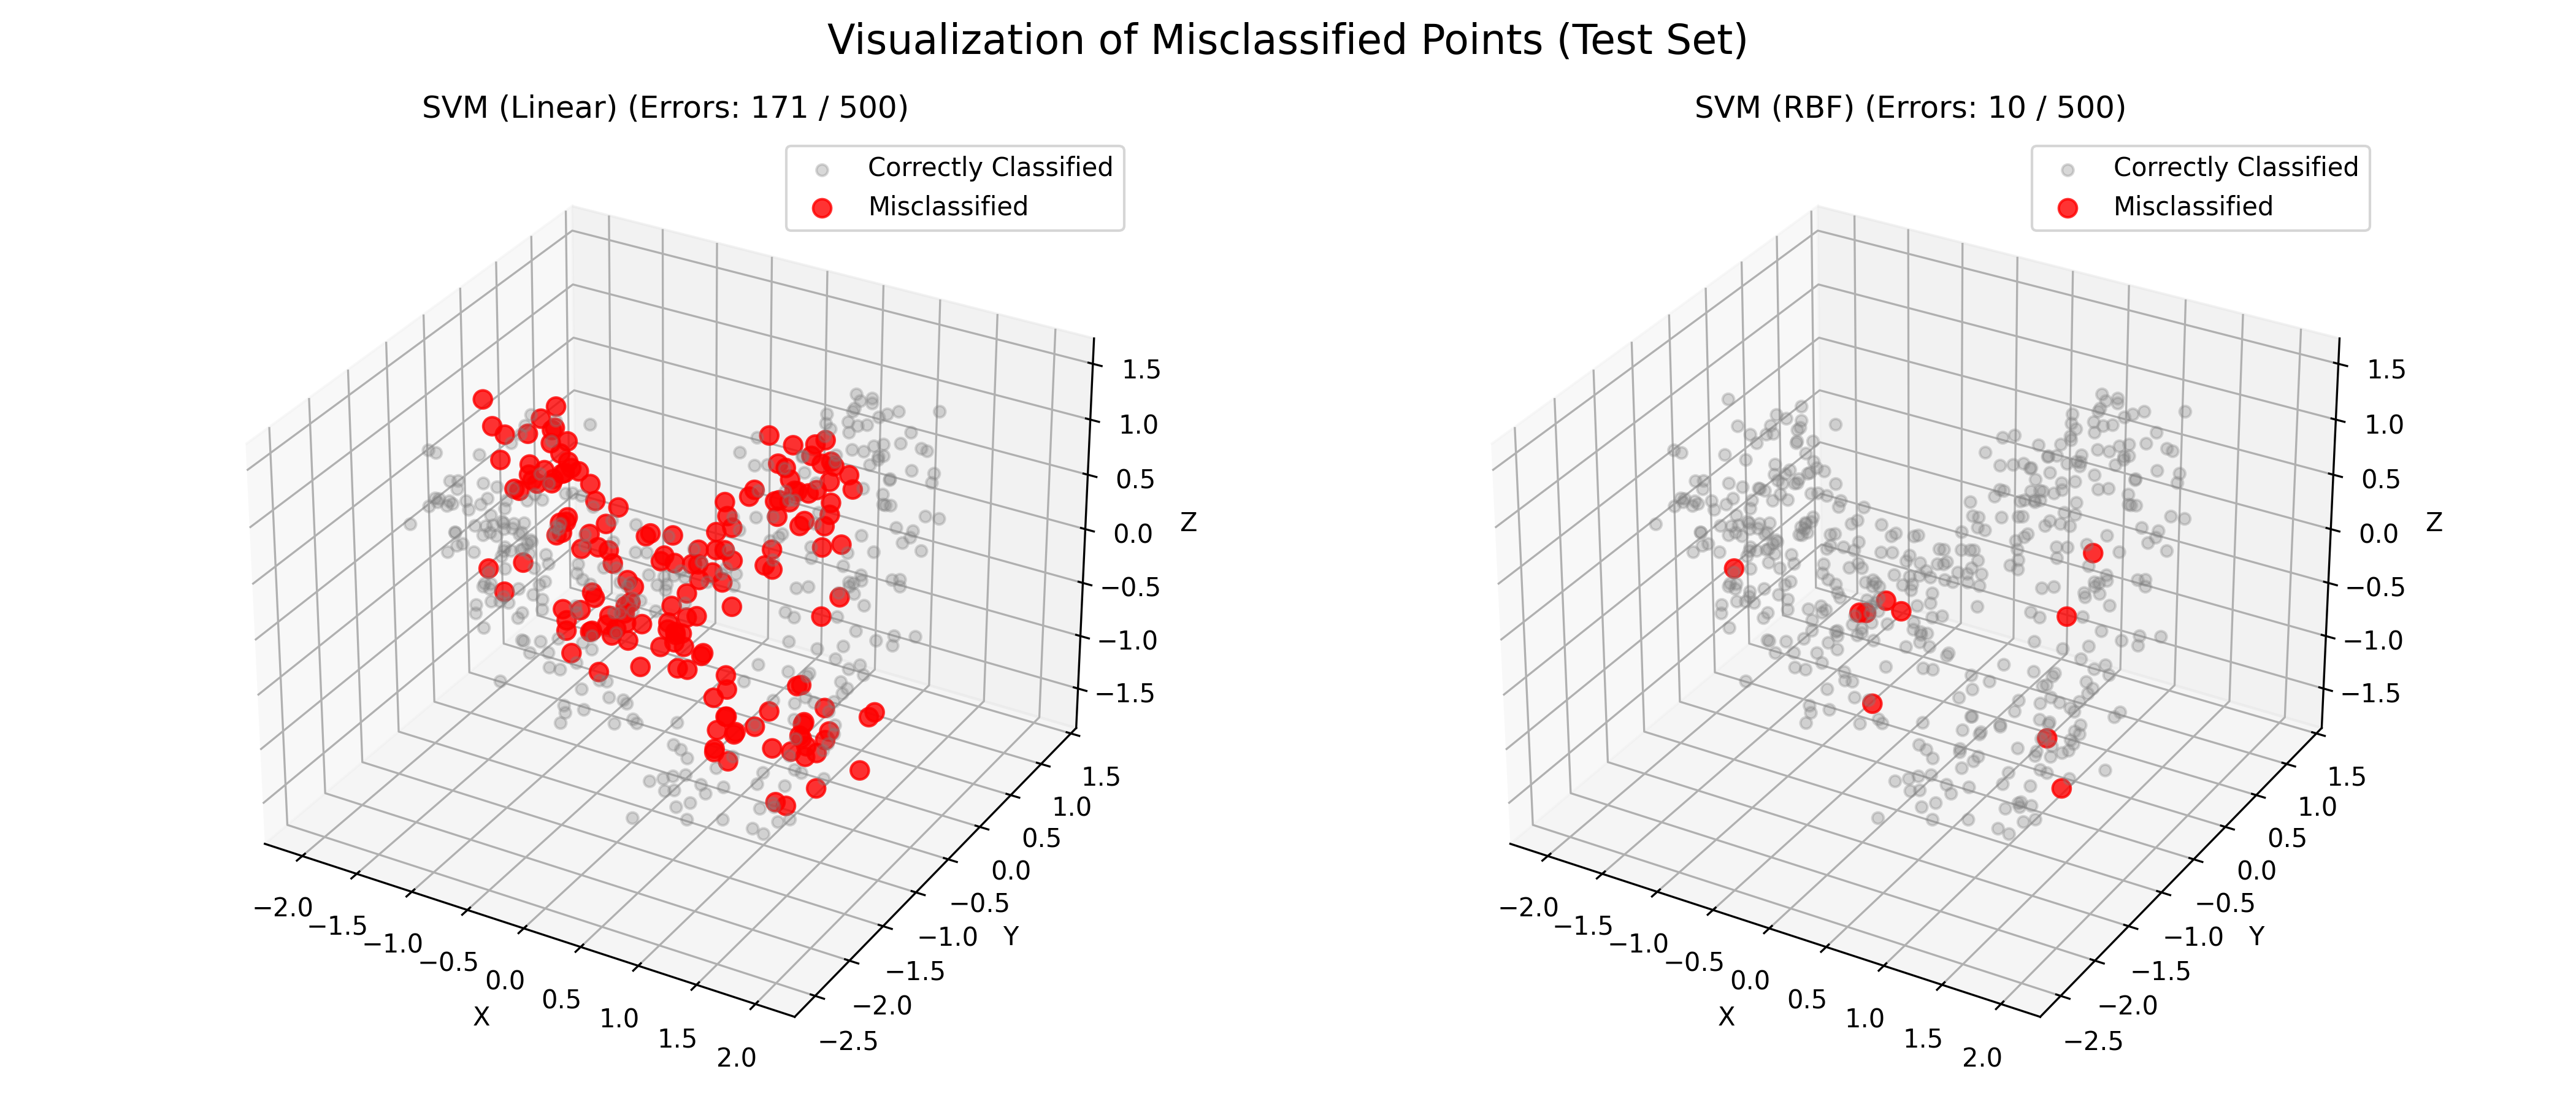
\includegraphics[width=0.85\textwidth]{error_visualization.png}
    \caption{\textbf{Spatial Distribution of Misclassified Points (Red)}}
    \label{fig:error_vis}
\end{figure}

\textbf{Spatial Analysis:}\\
\noindent The left panel (Linear SVM) clearly visualizes the inadequacy of a flat hyperplane; the errors form dense clusters where the "moons" interlock and curve sharply. Conversely, the right panel (RBF SVM) demonstrates that the algorithm almost perfectly captured the manifold structure. The very few errors remaining are isolated, stochastic artifacts entirely caused by the injected Gaussian noise, indicating that the RBF kernel has extracted the maximum possible underlying signal.

\subsection{Hyperparameter Sensitivity Analysis}
To fully unlock the potential of the RBF SVM, it is critical to briefly discuss the theoretical impact of its hyperparameters: the penalty parameter $C$ and the kernel coefficient $\gamma$. 
\begin{itemize}
    \item \textbf{Impact of $C$:} Controls the trade-off between achieving a low error on the training data and minimizing the model complexity. A very high $C$ forces the model to create convoluted boundaries just to correctly classify noise points (overfitting), while a low $C$ encourages a smoother, more generalized boundary.
    \item \textbf{Impact of $\gamma$:} Defines the radius of influence of a single training example. A large $\gamma$ makes the Gaussian bump narrow, making the decision boundary highly dependent on individual points. A smaller $\gamma$ broadens the bump, creating smoother regions. 
\end{itemize}
In our implementation, relying on the default parameters ($C=1.0$, $\gamma=\text{scale}$) already yielded a $98.00\%$ accuracy, proving that the default RBF manifold perfectly aligns with the fundamental geometry of the 3D Moons distribution.

\section{Conclusions}
The 3D Make Moons classification problem effectively exposes the architectural limitations of linear methods on complex topological data. While Decision Trees can capture non-linearity, their reliance on orthogonal splits and susceptibility to noise—even when ensembled via AdaBoost—can produce inconsistent reliability. Ultimately, algorithms equipped with localized, infinite-dimensional mapping mechanisms—specifically the SVM with an RBF Kernel—demonstrate unmatched proficiency in untangling non-linear manifolds. Through empirical accuracy metrics, detailed spatial error visualization, and confusion matrix analysis, we validate that the RBF Kernel provides the most robust generalization and structural adaptation.

\newpage
\phantomsection  % <--- 加上这一行，生成一个隐形锚点
\addcontentsline{toc}{section}{References}
\begin{thebibliography}{99}
    \bibitem{bishop2006} Bishop, C. M. (2006). \textit{Pattern Recognition and Machine Learning}. Springer.
    \bibitem{freund1997} Freund, Y., \& Schapire, R. E. (1997). \textit{A decision-theoretic generalization of on-line learning and an application to boosting}. Journal of computer and system sciences, 55(1), 119-139.
    \bibitem{boser1992} Boser, B. E., Guyon, I. M., \& Vapnik, V. N. (1992). \textit{A training algorithm for optimal margin classifiers}. In Proceedings of the fifth annual workshop on Computational learning theory (pp. 144-152).
\end{thebibliography}

\end{document}